\section{Code Validation}
A set of simulations was performed to evaluate the accuracy and reliability of Omnisoot in predicting soot formation. The aerosol dynamics models were validated by comparing the results of the population balance models implemented in Omnisoot with discrete element method (DEM) simulations reported in the literature. In addition, carbon and hydrogen mass and energy balances were rigorously assessed to ensure that residuals remain within the bounds of acceptable numerical error.


\section{Collision Frequency}
The collision frequency function determines the rate at which two particles collide, which results in the reduction of the total number of agglomerates and the increase in particle size. In the absence of strong flow shear or external forces, Brownian motion is the main driving force for particle coagulation. As explained in Sections~\ref{sec:seccoag} and \ref{sec:mpbm}, Omnisoot employs harmonic mean and Fuchs interpolations to calculate collision frequency of agglomerates from free-molecular ($\mathrm{Kn}\ge10$) to continuum ($\mathrm{Kn}\le0.1$) regimes based on gas mean free path and particle size. 


The test case for validation of collision frequency is based on the DEM simulation of 2000 monodisperse spherical particles with the density of 2200 $\mathrm{kg/m^3}$ in
a cubic cell with the constant temperature of 298 K and pressure of 1 atm~\citep{goudeli2015coagulation}. Figure~\ref{fig:kernelvalid} depicts the collision frequency plotted against Knudsen number (Kn$=2\lambda/d_m$) obtained by Omnisoot using harmonic mean (red solid line) and Fuchs interpolation (blue dashed line) and DEM results of \citet{goudeli2015coagulation}. The Fuchs interpretation perfectly matches DEM data over the free-molecular to the continuum range. Harmonic mean is also in good agreement with the DEM results in the free-molecular and continuum regimes, but slightly underpredicts the collision frequency in the transition regime (0.1$\le$Kn$\le$10) with relative errors less than 16\%.

\begin{figure}[H]
	\centering
	\begin{tikzpicture}
		\draw (0, 0) node[inner sep=0] 	{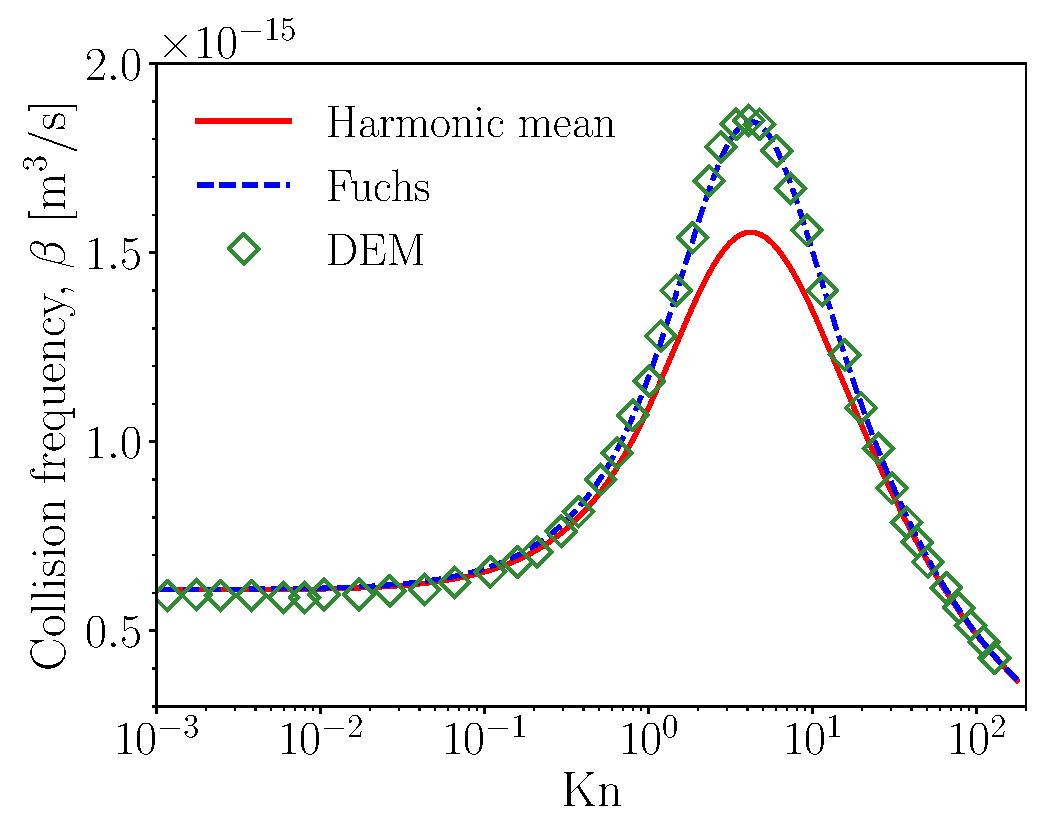
\includegraphics[width=0.45\textwidth]{Figures/Results/Validation/Kernel/kernel_valid.pdf}};
		\draw (-0.33, 1.11) node {\footnotesize{\cite{goudeli2015coagulation}}};
	\end{tikzpicture}
	\caption{The comparison of collision frequency, $\beta$, obtained by Omnisoot using harmonic mean (red solid line) and Fuchs interpolations (blue dashed line) with DEM results (symbols)~\citep{goudeli2015coagulation}}
	\label{fig:kernelvalid} 
\end{figure}



\subsection{Coagulation}
A test case\footnote{\href{https://github.com/mohammadadib-cu/omnisoot-cv/tree/main/validations/coagulation/free_molecular}{https://github.com/mohammadadib-cu/omnisoot-cv/tree/main/validations/coagulation/free\_molecular}} was set up to validate the coagulation sub-model of both particle dynamics models, MPBM and SPBM, in the free-molecular regime by comparing the results of Omnisoot with those of DEM~\citep{kholghy2021surface}. An adiabatic CVR with a volume of 1~$\mathrm{m}^3$ was initialized with $2.6261 \times 10^{18}$ spherical particles, each 2nm in diameter. The initial pressure and temperature of reactor are 1 atm and 1830 K, respectively. The particles collide in the free-molecular regime and grow in size through coagulation, without inception, surface growth, or oxidation. Figure~\ref{fig:coagvalid_Nd} demonstrates the evolution of ${N_{agg}}$, ${N_{pri}}$, ${d_m}$, and ${d_g}$ as predicted by MPBM and SPBM, which are in good agreement with DEM results~\citep{kholghy2021surface}. ${N_{pri}}$ is conserved during coagulation, resulting in identical flat trends for both models. In contrast, ${N_{agg}}$ decreases over time, with a faster decay observed in SPBM due to its treatment of agglomerate polydispersity, which leads to a higher collision frequency compared to MPBM. Therefore, $d_m$ and $d_g$  predicted by SPBM, shown in Figure~\ref{fig:coagvalid_Nd}b, are slightly larger than those predicted by MPBM.

\begin{figure}[H]
	\centering
	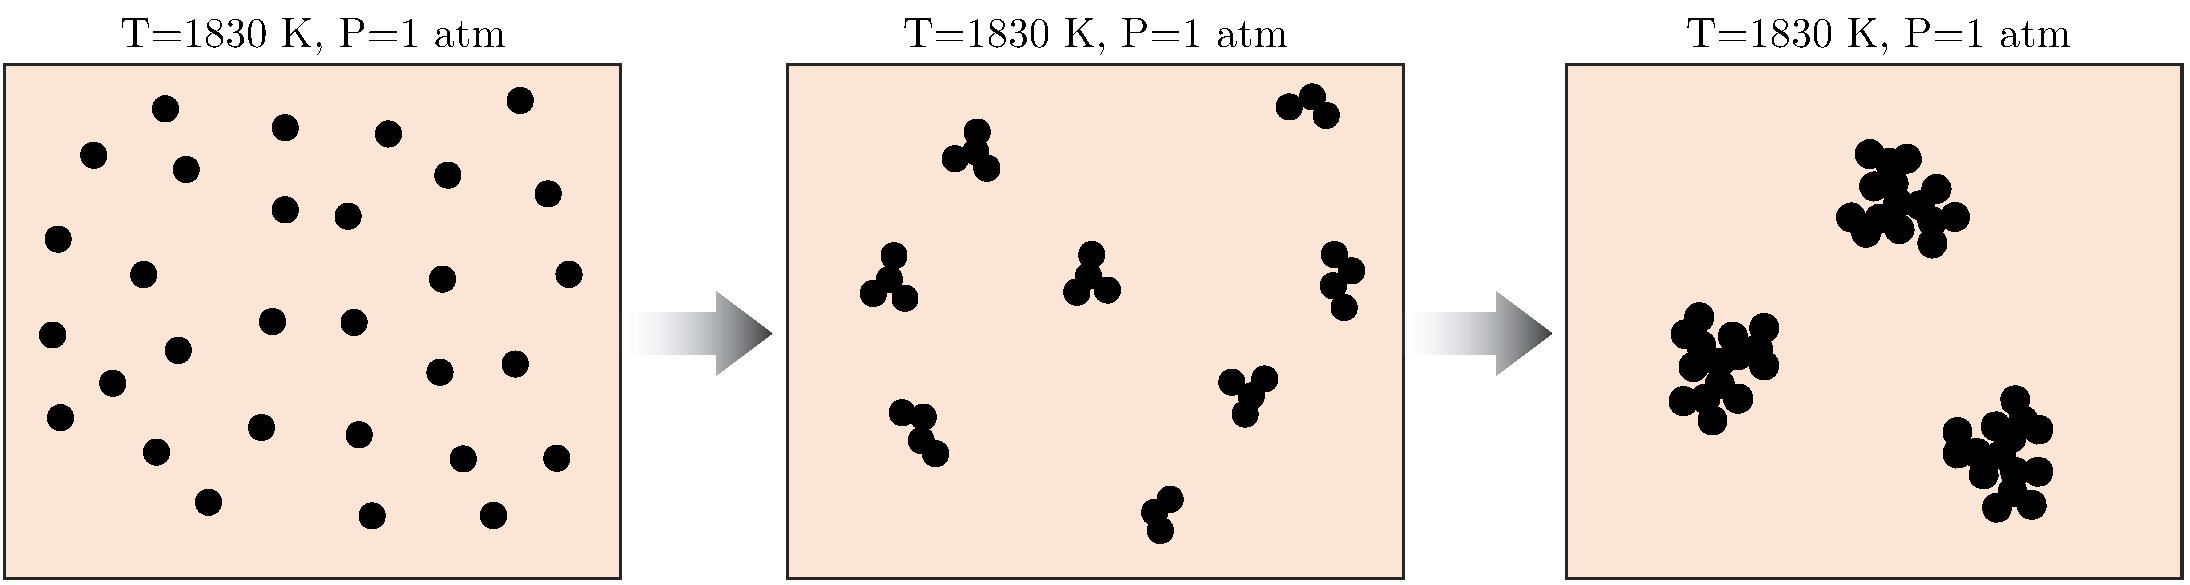
\includegraphics[width=0.9\textwidth]{Figures/Results/Validation/Coagulation/coagulation_scheme.pdf}
	\caption{The schematic of the agglomeration process in the coagulation test case where initially spherical particles collide and form agglomerates}
	\label{fig:coagscheme}
\end{figure}

The MPBM model cannot resolve the particle size distribution (PSD) due to the monodispersity assumption. In contrast, the SPBM tracks the number concentration of particles in discrete sections, allowing the construction of an evolving PSD, calculation of mean properties, and assessment of the size distribution spread during coagulation. Figure~\ref{fig:coagvalid_sigmapsd}a shows the standard deviation of the mobility diameter, ${\sigma_g}$, predicted by SPBM, which is in close agreement with DEM results. Initially, ${\sigma_g}=1$, indicating a monodisperse population, and it gradually increases, reaching a final value of 2.03, which corresponds to the characteristic standard deviation for the free-molecular regime~\citep{vemury1995self}.

Figure~\ref{fig:coagvalid_sigmapsd} shows the evolution of the non-dimensional particle size distribution (PSD) from $t=$1 ms to 680 ms. The PSD is plotted as a function of the normalized concentration, ${\Psi= \bar{v}n_{agg}(v,t)/N_{agg,\infty}}$ and dimensionless volume, ${\eta= v/ \bar{v}}$, where ${n_{agg}(v,t)}$ is the size distribution function of agglomerate, ${v}$ is particle volume, ${\bar{v}}$ is mean particle volume, ${N_{agg,\infty}}$ is the total number concentration of agglomerates. At short residence times ($t\approx4$ ms), the PSD resembles a half bell curve because the majority of particles have sizes close to ${d_0=}$2 nm, and the average particle volume is close to the minimum volume, resulting in the highest concentration occurring at ${\eta\approx1}$. As particles grow through coagulation, the PSD rapidly evolves into a full bell curve ($\mathrm{t\ge}$22 ms) and remains unchanged at longer residence times ($\mathrm{t\ge}$450 ms), indicating the attainment of a self-preserving size distribution (SPSD). This behavior is in good agreement with DEM results and confirms the capability of the SPBM implemented in Omnisoot to capture SPSD for soot agglomerates, a characteristic outcome of Brownian-driven particle coagulation.

%\begin{table}
%	\caption{The simulations conditions of the coagulation test case~\citep{kholghy2021surface}}
%	\label{tab:simcond_coagtest}
%	\centering
%	\begin{tabular}{l l}
%		\hline
%		\textbf{Property} & \textbf{Value} \\
%		\hline
%		Composition & $\mathrm{CH_4}$:0.425, $\mathrm{O_2}$:0.435, $\mathrm{N_2}$:0.14\\
%		T & 1830 K\\
%		P & 1 atm \\
%		${N^1_{agg}}$ & $3.514\times10^{-5} \mathrm{mol/kg}$ \\ 
%		${N^1_{pri}}$ & $3.514\times10^{-5} \mathrm{mol/kg}$\\
%		${d^1_{p}}$ & 2 nm \\
%		\hline
%	\end{tabular}
%\end{table}


\begin{figure}[H]
	\centering
	\begin{subfigure}[t]{0.4\textwidth}
		\begin{tikzpicture}
			\draw (0, 0) node[inner sep=0] 	{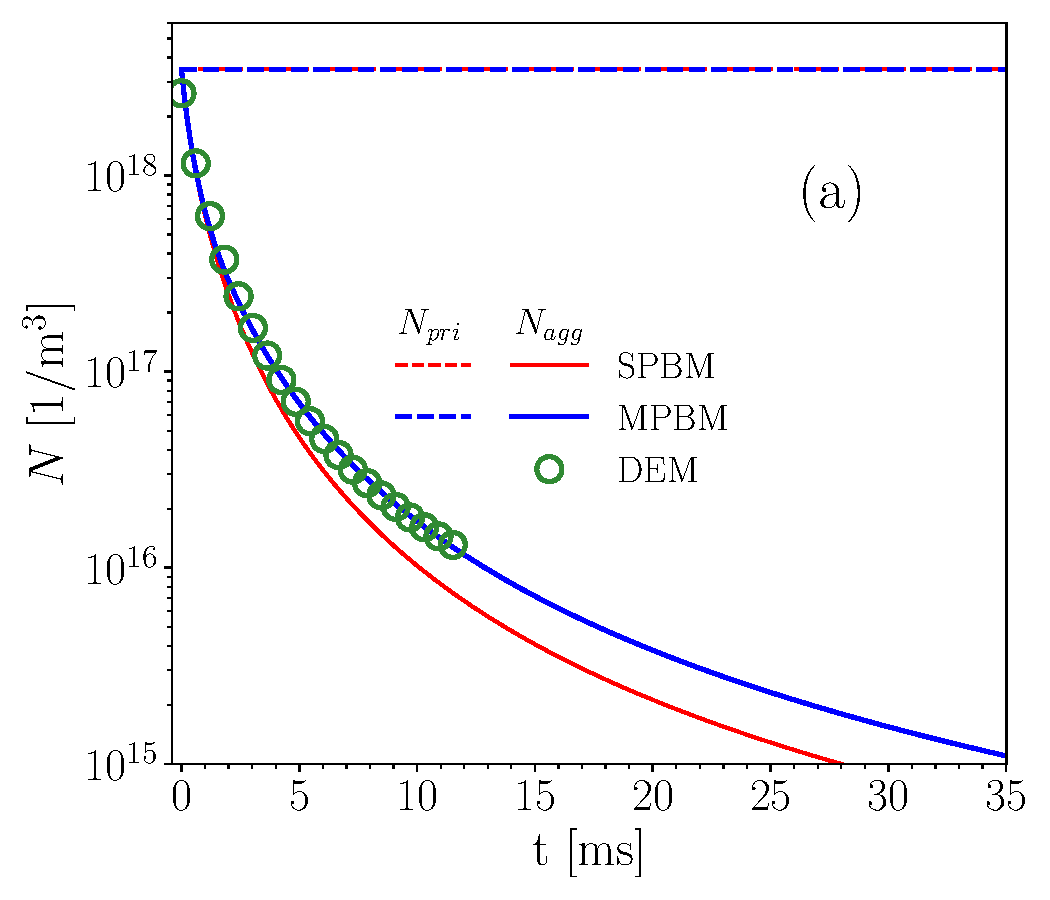
\includegraphics[width=1\textwidth]{Figures/Results/Validation/Coagulation/N_agg_pri.pdf}};
			\draw (2.1, 0.03) node {\scriptsize{\cite{kholghy2021surface}}};
		\end{tikzpicture}
	\end{subfigure}
	\begin{subfigure}[t]{0.4\textwidth}
		\begin{tikzpicture}
			\draw (0, 0) node[inner sep=0] 	{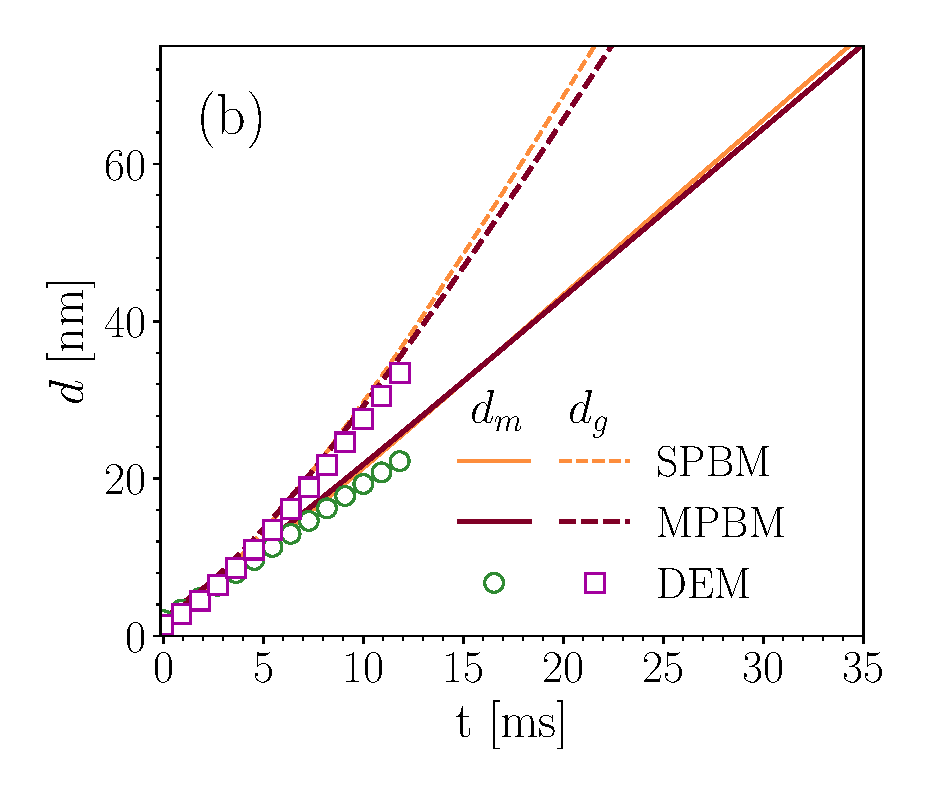
\includegraphics[width=1\textwidth]{Figures/Results/Validation/Coagulation/d_mg.pdf}};
			\draw (2.2, -1.22) node {\scriptsize{\cite{kholghy2021surface}}};
		\end{tikzpicture}
	\end{subfigure}
	\caption{The number concentration of agglomerates and primary particles (a), and mobility and gyration diameters (b) obtained by Omnisoot using MPBM and SPBM, which are in close agreement with the DEM results~\citep{kholghy2021surface} indicating the validation of the coagulation sub-models}
	\label{fig:coagvalid_Nd} 
\end{figure}


\begin{figure}[H]
	\centering
	\begin{subfigure}[t]{0.4\textwidth}
		\begin{tikzpicture}
			\draw (0, 0) node[inner sep=0] 	{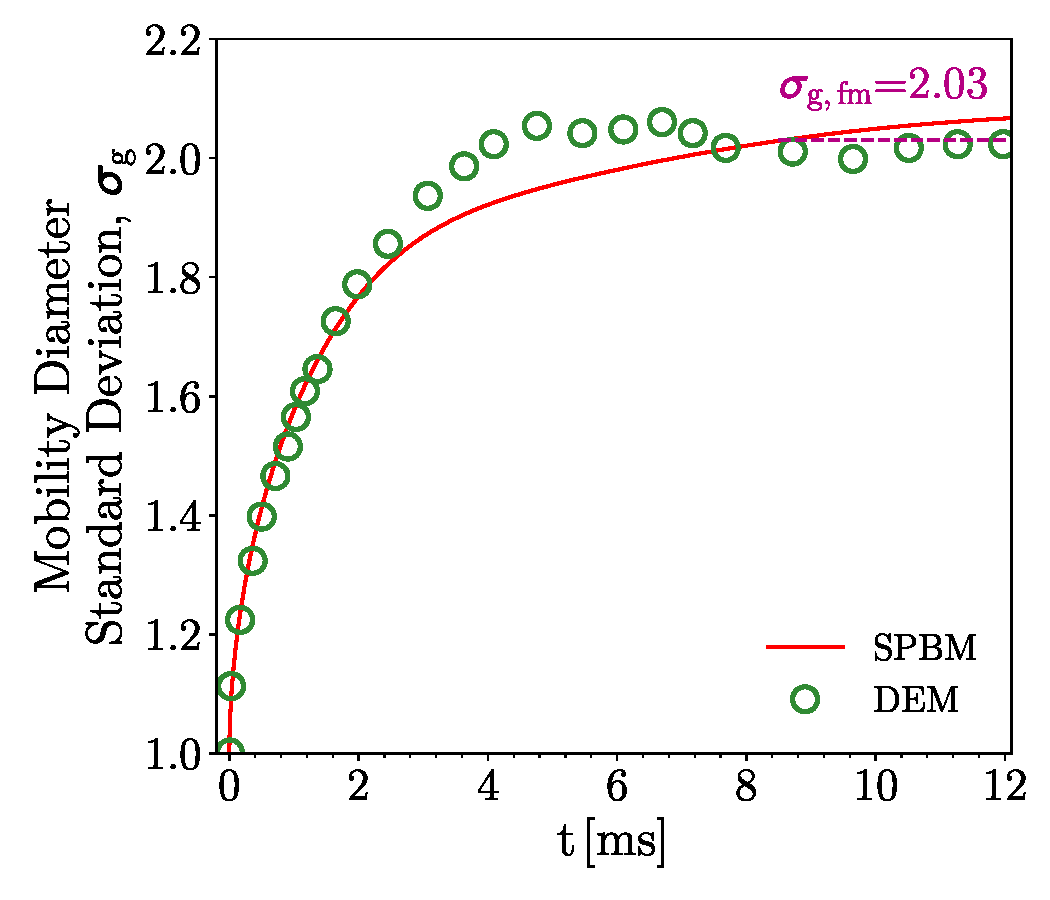
\includegraphics[width=1\textwidth]{Figures/Results/Validation/Coagulation/sigmag.pdf}};
			\draw (0.54, -1.02) node {\scriptsize{\cite{kholghy2021surface}}};
		\end{tikzpicture}
	\end{subfigure}
	\begin{subfigure}[t]{0.4\textwidth}
		\begin{tikzpicture}
			\draw (0, 0) node[inner sep=0] 	{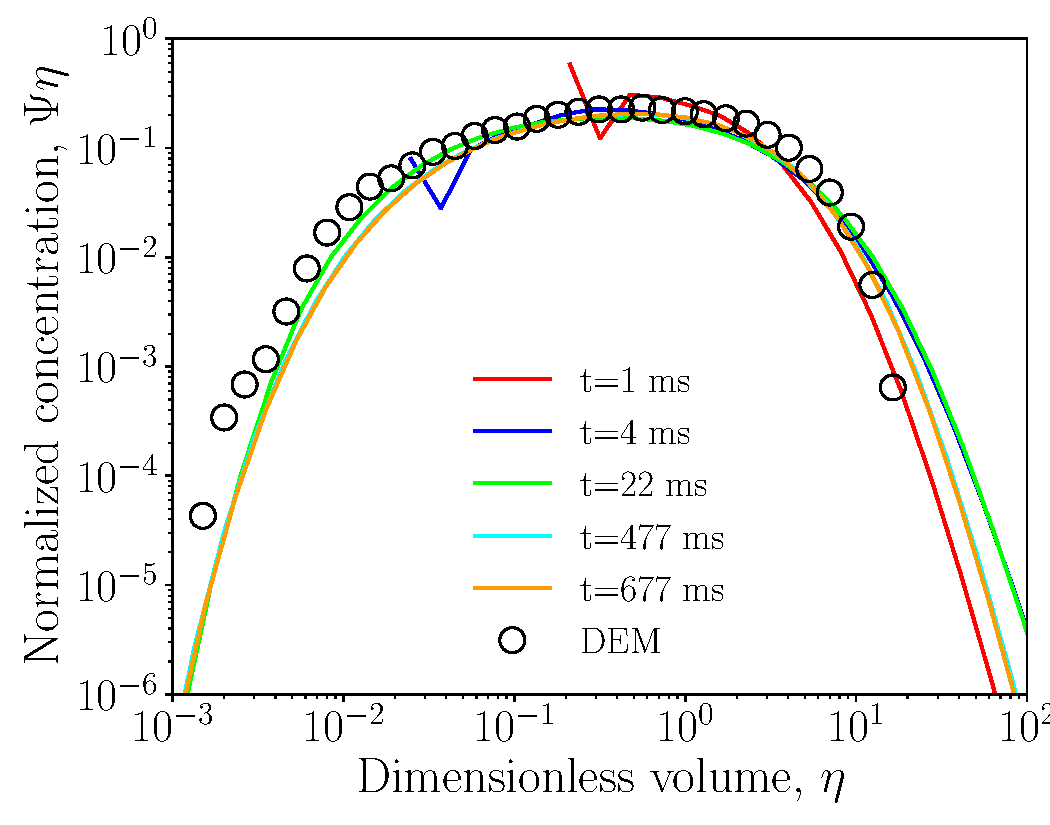
\includegraphics[width=1\textwidth]{Figures/Results/Validation/Coagulation/PSD.pdf}};
			\draw (1.3, -1.2) node {\scriptsize{\cite{goudeli2015coagulation}}};
		\end{tikzpicture}
	\end{subfigure}
	\caption{Standard deviation of the mobility diameter, $\mathrm{\sigma_g}$, obtained by SPBM is in close agreement with DEM results~\citep{kholghy2021surface} (a). The non-dimensional particle size distribution at different residence times (b) overlaps after the initial transient phase, indicating the attainment of a self-preserving size distribution, which is also in good agreement with DEM results~\citep{goudeli2015coagulation}.}
	\label{fig:coagvalid_sigmapsd} 
\end{figure}

A similar test\footnote{\href{https://github.com/mohammadadib-cu/omnisoot-cv/tree/main/validations/coagulation/continuum}{https://github.com/mohammadadib-cu/omnisoot-cv/tree/main/validations/coagulation/continuum}} was performed in the continuum regime, and the results from the SPBM were compared with those obtained from DEM. The simulation conditions were the same as in the previous case, except for the temperature, $T = 600$ K, and the initial particle diameter, $d^1_p = 259$ nm. Figure~\ref{fig:coagvalid_contpsd} shows that the non-dimensional size distribution predicted by SPBM reaches the self-preserving state in good agreement with DEM results~\citep{goudeli2015coagulation}, which supports the validity of the coagulation sub-model in Omnisoot under continuum conditions.

\begin{figure}[H]
	\centering
	\begin{tikzpicture}
		\draw (0, 0) node[inner sep=0] 	{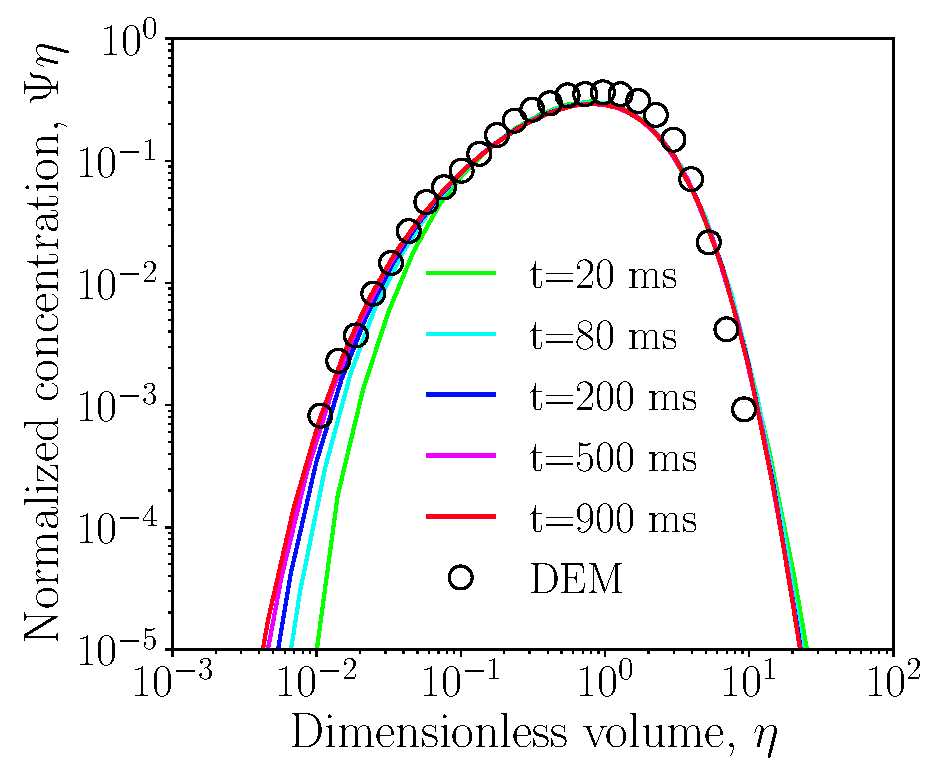
\includegraphics[width=0.4\textwidth]{Figures/Results/Validation/Coagulation/PSD_cont.pdf}};
		\draw (1.3, -1.22) node {\scriptsize{\cite{kholghy2021surface}}};
	\end{tikzpicture}
	\caption{The particle size distribution normalized number concentration of agglomerates plotted against non-dimensional volume reaches self-preserving size distribution in good agreement with DEM results~\citep{goudeli2015coagulation}}
	\label{fig:coagvalid_contpsd} 
\end{figure}


\subsection{Elemental and Energy Balance}
To ensure the accuracy and reliability of the simulations, the conservation of elemental mass and energy was assessed across all reactor models implemented in Omnisoot. Elemental balances of carbon and hydrogen, as well as the total energy (internal or enthalpy depending on the reactor type) of the gas-particle system, were evaluated during soot formation processes under various pyrolysis and combustion conditions.

\subsubsection{Constant Volume Reactor}
The pyrolysis of 30\% $\mathrm{CH_4}$ diluted in $\mathrm{N_2}$ with the initial temperature and pressure of 2455 K and 3.47 atm, respectively, was simulated using CVR with a residence time of 40 ms. The combination of available PAH growth and particle dynamics models results in eight different cases, which were simulated to verify conservation of mass and energy. Here, we focus on the total elemental balance of carbon and hydrogen, as they are key elements involved in soot formation.
Figure~\ref{fig:constuvvalid} shows the relative errors in total carbon, hydrogen, and energy for the different PAH growth and particle dynamics models. In all cases, the errors fall below $\mathrm{10^{-10}}$, confirming that CVR satisfies mass and energy conservation.

\begin{figure}[H]
	\centering
	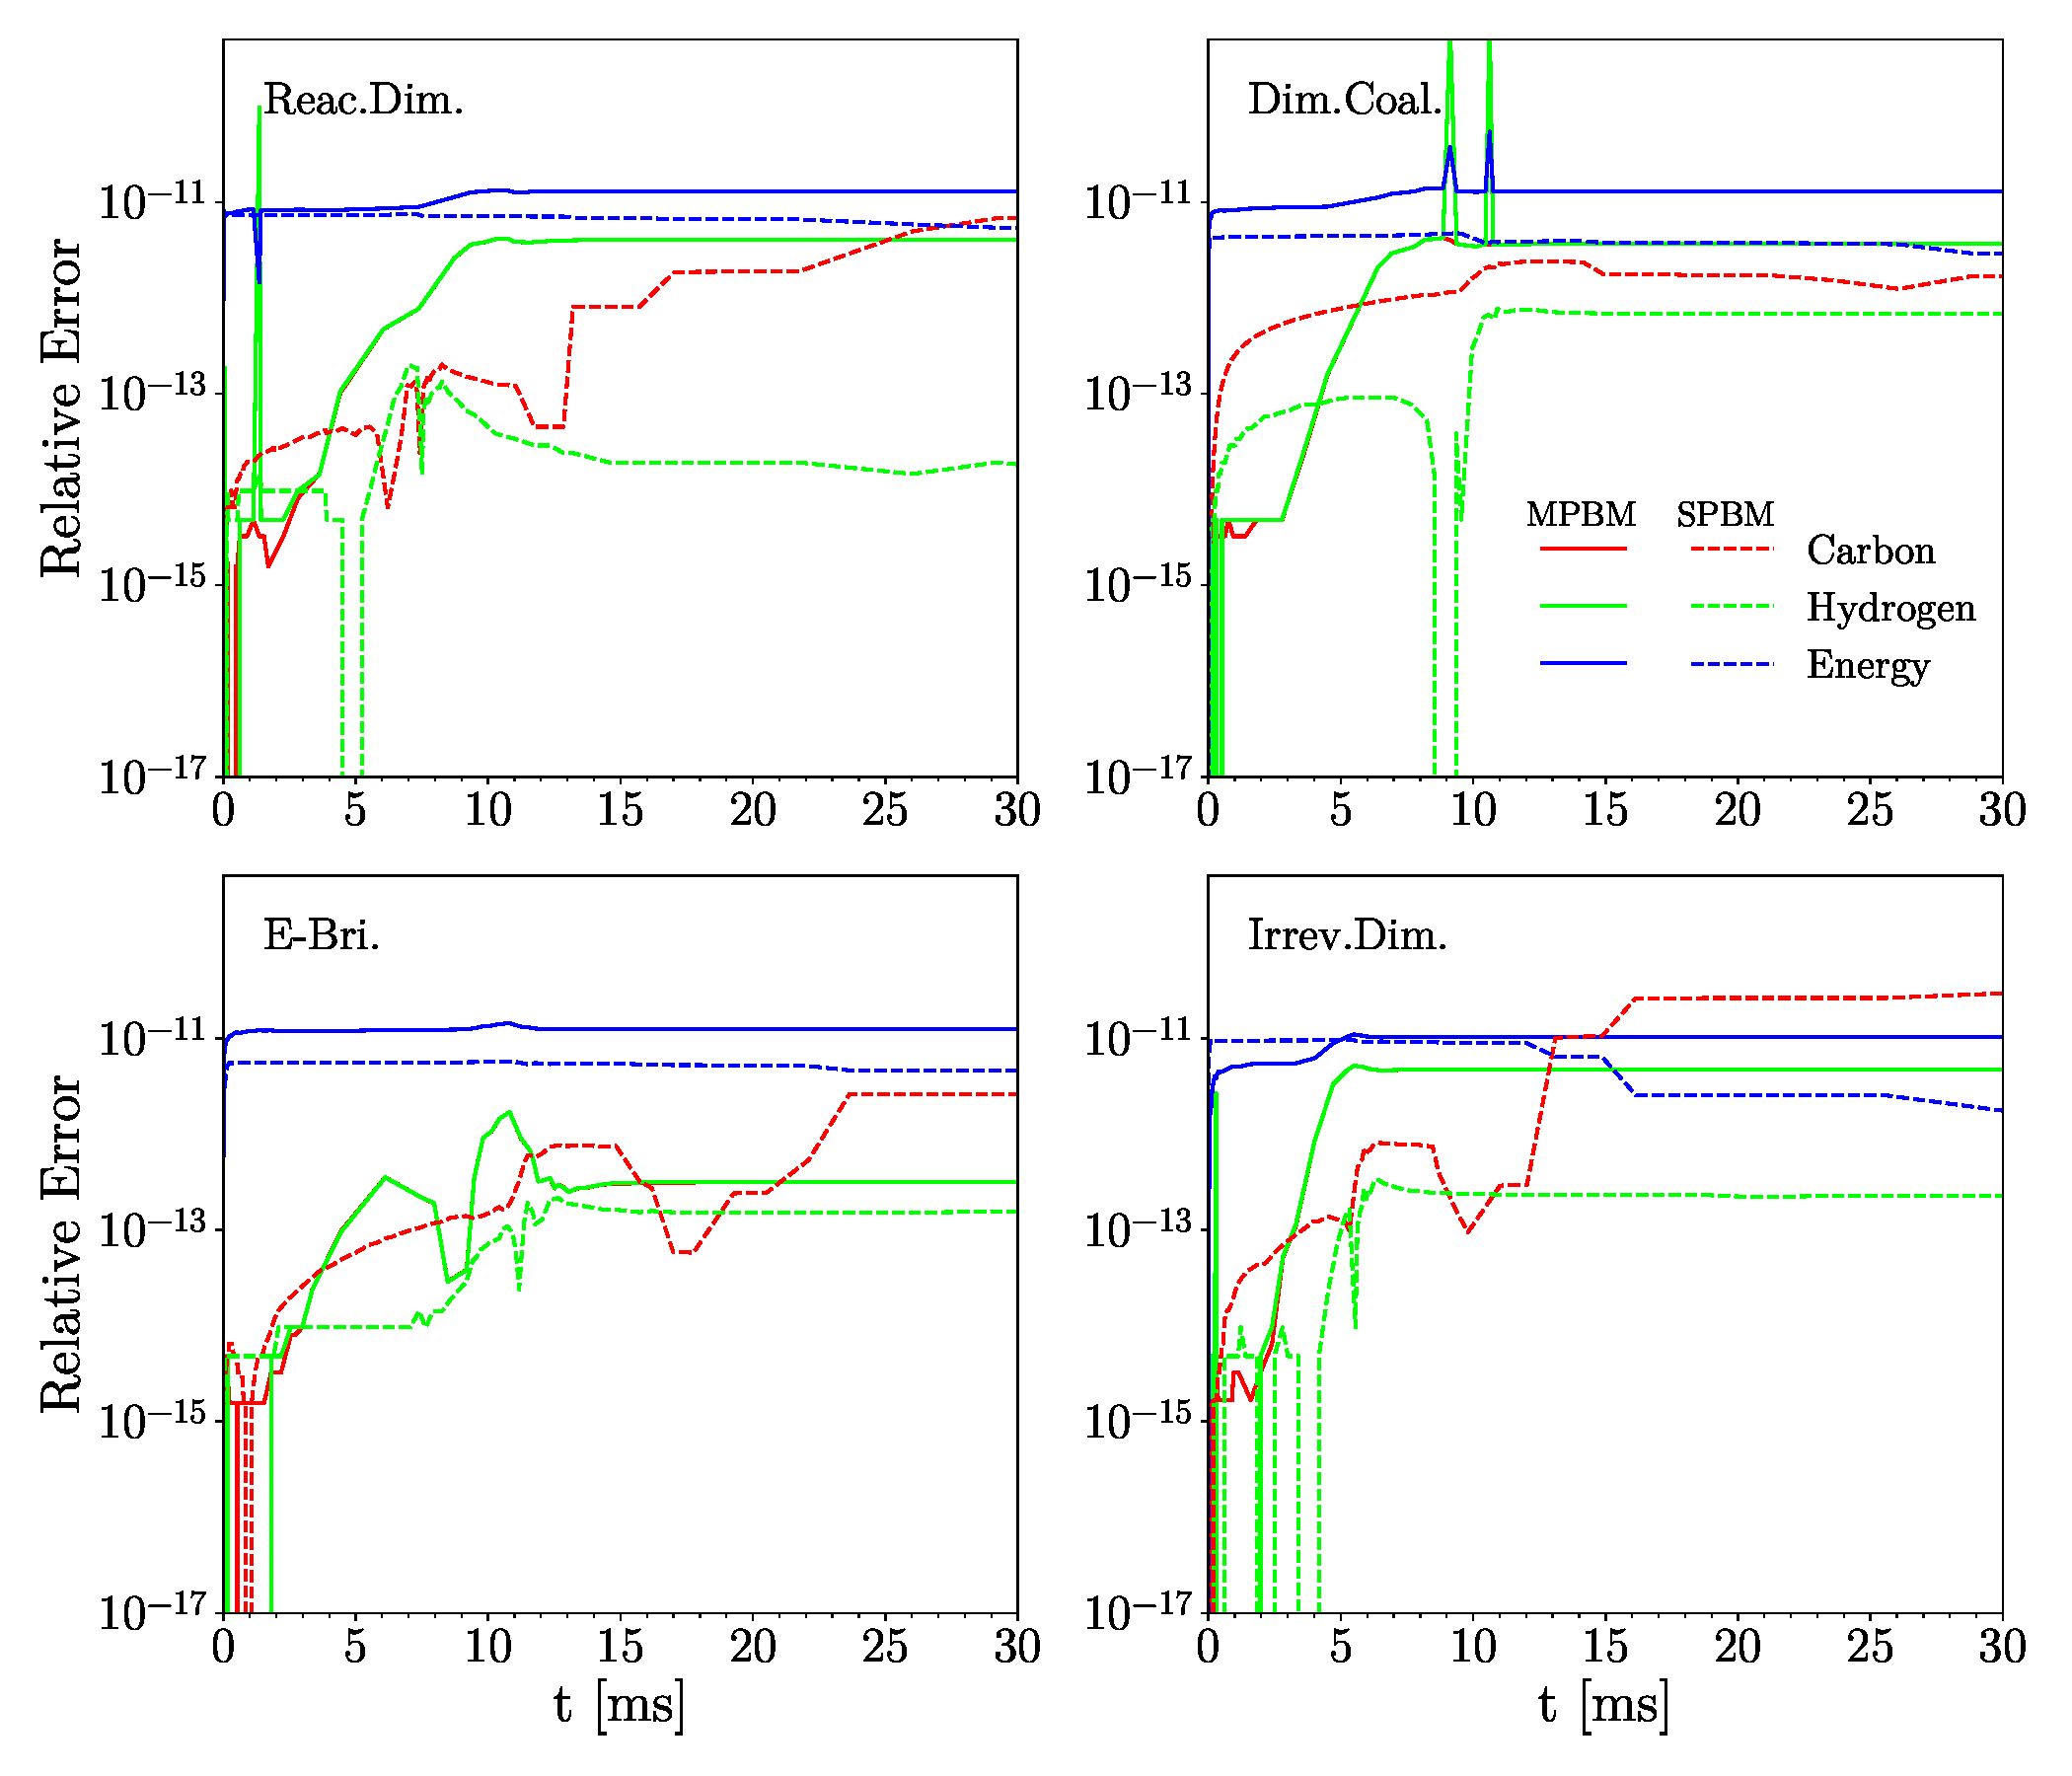
\includegraphics[width=0.8\textwidth]{Figures/Results/Validation/ConstUV/relerr_constuv.pdf}
	\caption{The relative error of total carbon (red line) and hydrogen (green line) mass, and total internal energy residual of gas and soot (blue line) plotted against residence time during pyrolysis of 30\% $\mathrm{CH_4}$-$\mathrm{N_2}$ at 2455 K and 3.47 atm in the constant volume reactor simulated using different PAH growth models along with MPBM (solid line) and SPBM (dashed line)}
	\label{fig:constuvvalid}
\end{figure}

\subsection{Imposed Pressure Reactor}

The pyrolysis of 5\%$ \mathrm{CH_4}$ in a shock-tube at post-reflected-shock temperature and pressure of $\mathrm{T_5}=$2355 K and $\mathrm{P_5}=4.64$ atm was simulated using IPR model. The pressure was measured using an end-wall sensor by the Hanson Research Group at Stanford University. Details of the experimental setup are provided in Sec.\ref{sec:shockexpsetup}. The measured pressure signal was smoothed using the Savitzky–Golay filter in SciPy\citep{2020SciPy} to reduce fluctuations in the raw signal and make it suitable for the numerical solver. The residual of carbon and hydrogen mass are less than $10^{-12}$, while the energy residual reaches up to $10^{-6}$ for energy by the end of the simulation. The relatively higher energy residual is attributed to pressure work.
\begin{figure}[H]
	\centering
	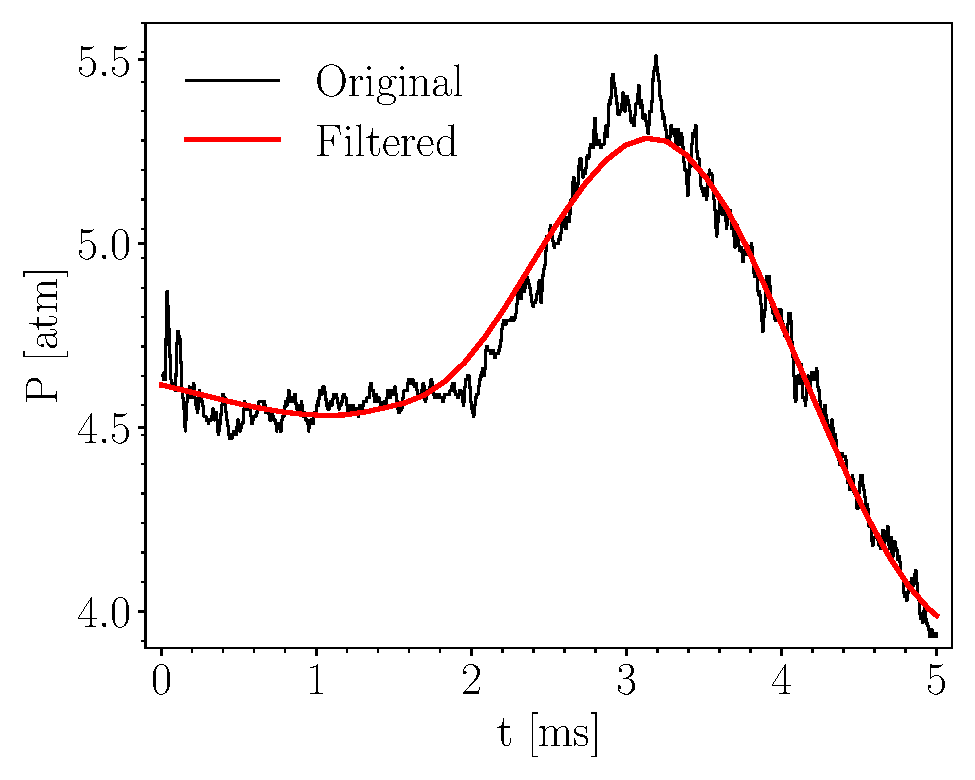
\includegraphics[width=0.4\textwidth]{Figures/Results/Validation/IPR/pressure.pdf}
	\caption{The pressure time history (black line) measured by the Stanford group for pyrolysis of 5\%$\mathrm{CH_4}$ at $\mathrm{T_5}=$2355 K and $\mathrm{P_5}=4.64$ atm, and filtered (red line) with reduced fluctuations used to specify the pressure of the reactor}
	\label{fig:iprpressurevalid}
\end{figure}


\begin{figure}[H]
	\centering
	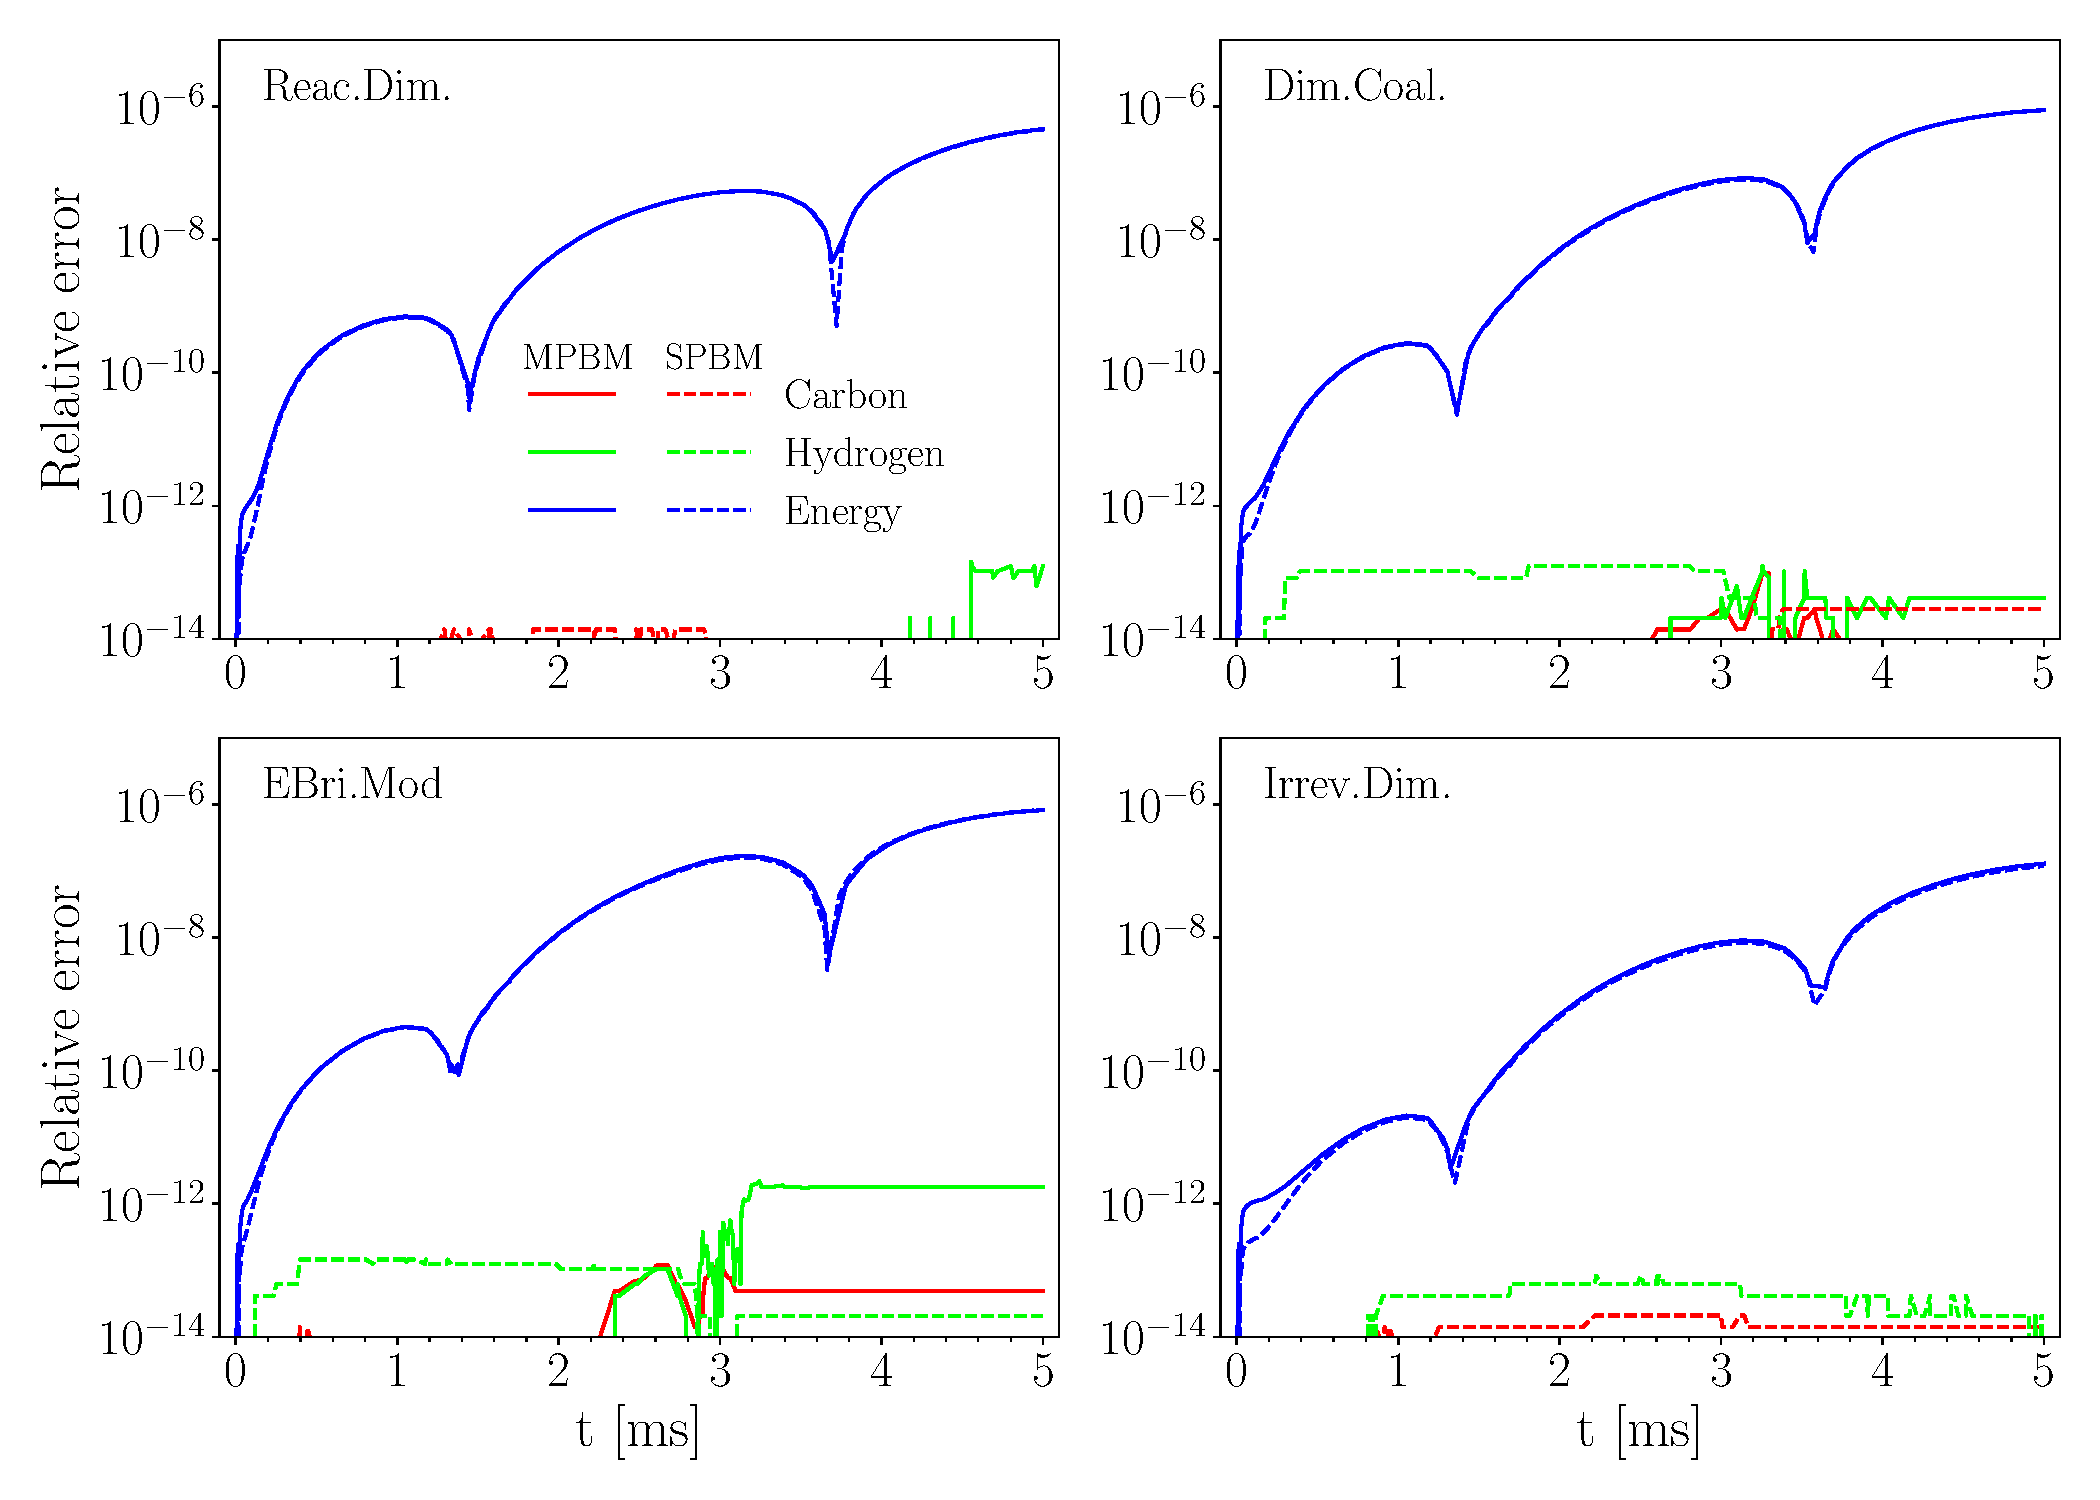
\includegraphics[width=0.8\textwidth]{Figures/Results/Validation/IPR/relerr_pressure.pdf}
	\caption{The relative error of total carbon (red line) and hydrogen (green line) mass, and total internal energy residual of gas and soot (blue line) plotted against residence time during pyrolysis of 5\% $\mathrm{CH_4}$-Ar at post-reflected-shock temperature and pressure of $\mathrm{T_5}=$2355 K and $\mathrm{P_5}=4.64$ atm with an imposed pressure profile simulated using different PAH growth models along with MPBM (solid line) and SPBM (dashed line)}
	\label{fig:iprvalid}
\end{figure}


\subsection{Perfectly Stirred Reactor}
\label{sec:psrvalid}
The mass and energy balance are investigated for soot formation during ethylene-air oxidation at equivalence ratio of $\phi=2$ in a perfectly stirred reactor. The simulation conditions were chosen based on the combustor implemented and utilized by \citet{stouffer2002combustion}. The reactants enter the reactor with the volume of 250 ml at 300 K and atmospheric pressure. The simulation is initialized from a high temperature ($\approx$2000 K) to avoid trivial solution (cold reactant leaving the reactor with no chemical reactions) and to ensure the model captures a sustained combustion. The residence time of products in the reactor is 8.5 ms. Figure~\ref{fig:psrvalid} shows the relative error of total elemental carbon and hydrogen mass and total enthalpy of gas and soot, which is less than $10^{-6}$ for all combinations of particle dynamics and PAH growth models.

\begin{figure}[H]
	\centering
	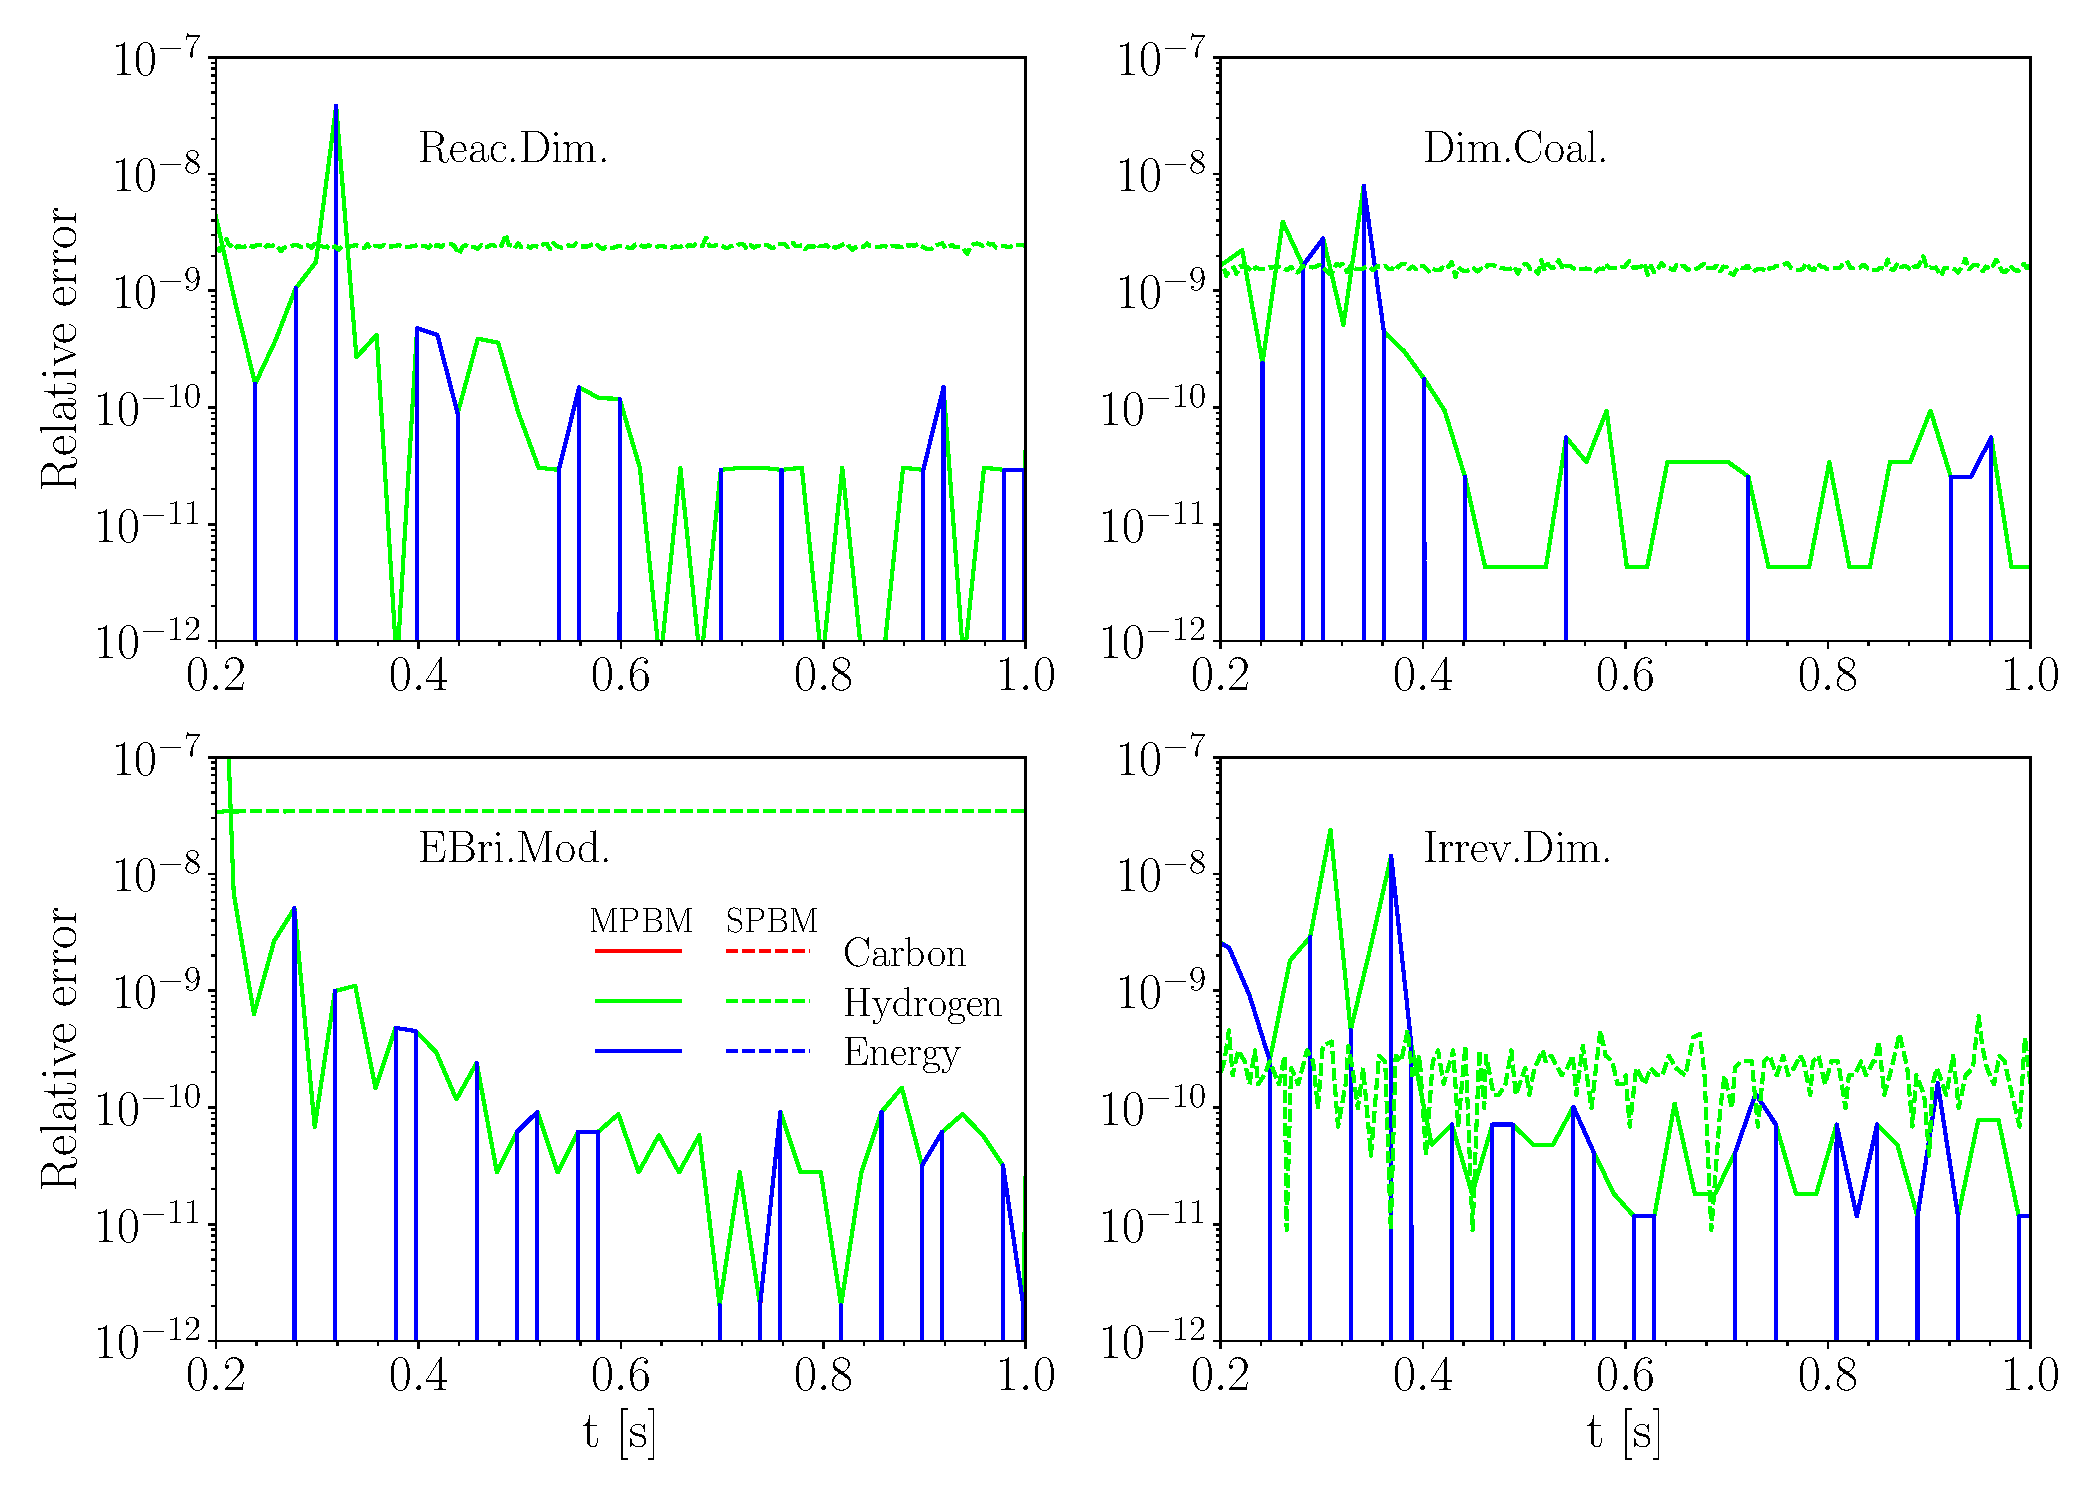
\includegraphics[width=0.8\textwidth]{Figures/Results/Validation/PSR/relerr_psr.pdf}
	\caption{The relative error of total carbon (red line) and hydrogen (green line) mass, and total internal energy residual of gas and soot (blue line) plotted in simulation time during adiabatic combustion of $\mathrm{C_2H_4}$-air with $\phi=2$ at 1 atm simulated using different combinations of PAH growth models and particle dynamics models: MPBM (solid line) and SPBM (dashed line).}
	\label{fig:psrvalid}
\end{figure}

\subsection{Plug Flow Reactor}
Methane pyrolysis in an adiabatic PFR was used to assess the conservation of elemental carbon, hydrogen, and energy. The inlet stream 30\% $\mathrm{CH_4}$ diluted in $\mathrm{N_2}$ with an initial temperature of 2100 K and pressure of 1 atm. Figure~\ref{fig:pfrvalid} shows the residuals of total elemental carbon, hydrogen, and energy along the reactor length, up to 40 cm, for all combinations of PAH growth and particle dynamics models. The residuals remain below $10^{-11}$, confirming that the PFR model in Omnisoot satisfies mass and energy conservation.




\begin{figure}[H]
	\centering
	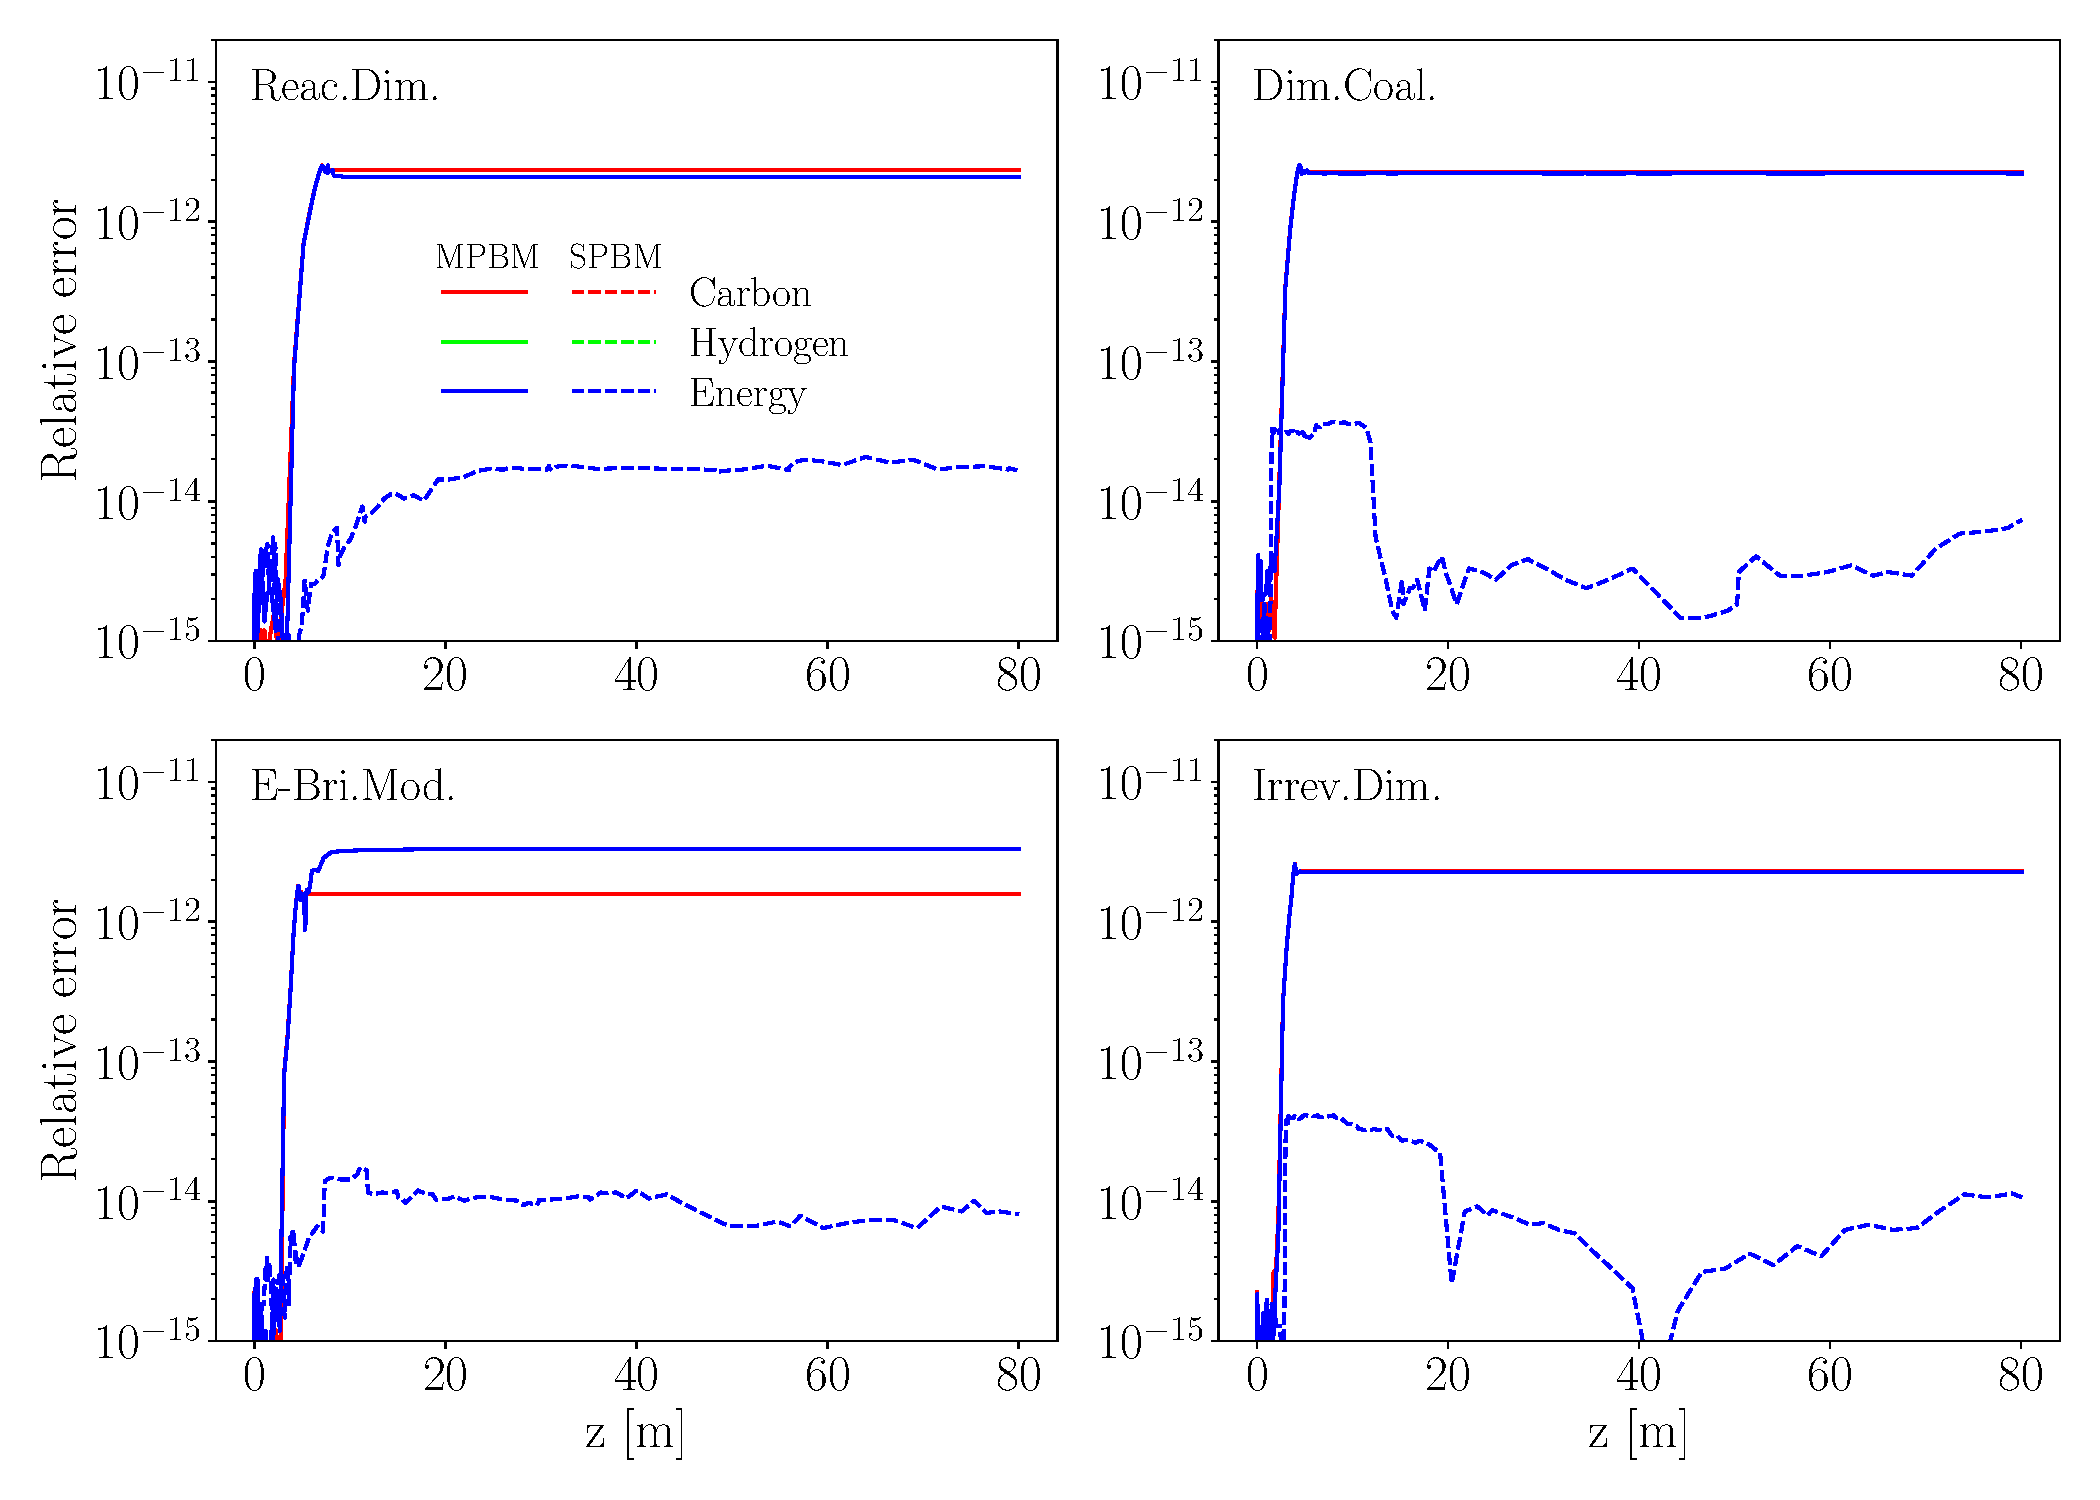
\includegraphics[width=0.8\textwidth]{Figures/Results/Validation/PFR/relerr_pfr.pdf}
	\caption{The relative error of total carbon (red line) and hydrogen (green line) mass, and total internal energy residual of gas and soot (blue line) plotted against reactor length (cm) in the adiabatic flow reactor during pyrolysis of 30\% $\mathrm{CH_4}$-$\mathrm{N_2}$ at 2100 K and 1 atm simulated using different PAH growth models and MPBM (solid line) and SPBM (dashed line)}
	\label{fig:pfrvalid}
\end{figure}